Tato část diplomové práce popisuje návrh aplikace pro podporu automatické správy virtualizačního kontejneru Solaris Zones na
platformě Solaris. Zaměřuje se především na popis funkcionality a požadavků, které aplikace musí splňovat. V~závěrečné části
této kapitoly je rozebrána bezpečnost a požadavky na~uživatele, který aplikaci bude moci využívat.
\section{Požadavky na aplikaci}
\label{chapter:design:demands}
Hlavním cílem této práce je vytvořit aplikaci, která bude administrátorovi operačního systému Solaris ulehčovat správu
většího množství neglobálních zón. Na základě účelu aplikace je nutné vytvořit požadavky, které bude muset výsledná implementace
aplikace splňovat. Pokud vytvořená aplikace splní stanovené požadavky, bude moci být cíl práce považován za splněný.

Jak bylo uvedeno výše, virtualizační technika Solaris Zones je exkluzivním produktem pro operační
systém Solaris. Tomuto faktu musí být přizpůsoben výběr technologií, které budou použity při implementaci výsledné aplikace.
Operační systém Solaris není standardní platformou, i když je v~dnešní době podporován na více platformách platformě. Hlavní důraz
musí být kladen na kompatibilitu programovacího jazyka a jeho knihoven s~operačním systémem Solaris. Z~výše uvedených důvodů
je možné vyvodit první požadavek na administrační nástroj, kterým je podpora na operačním systému \textbf{Solaris}.

Účelem nástroje má být podpora automatické správy neglobálních zón. Pod pojmem správa je myšlena podpora základních administračních
postupů a technik, které jsou z~velké části popsány v~kapitole \ref{chapter:zones}. Mezi tyto postupy patří 
vytváření neglobálních zón, ale také podpora jejich správy, zálohování nebo migrace. Automatickou správou je myšlena hlavně
automatizace procesů vytváření zóny, zálohy nebo migrace, které se skládají z~několika kroků. Aplikace by měla administrátorovi
poskytovat funkce, které umožní provedení výše zmíněných procesů pomocí jednoho příkazu. Požadavky na aplikaci vyplývající
z~účelu nástroje je možné specifikovat jako \textbf{podpora správy} Solaris Zones a~\textbf{automatizace procesů} administrace.

Virtualizační technika Solaris Zones poskytuje administrátorovi skrze příkazy \verb|zonecfg(1)| a \verb|zoneadm(1)| způsob,
jak spravovat lokální neglobální zóny. Zcela zde však chybí podpora pro správu zón na vzdálených serverech. V~dnešních infrastrukturách
počítačových systémů využívajících virtualizace se nachází mnoho serverů. Tyto servery poskytují své výpočetní prostředky
virtuálním strojům. Z~tohoto pohledu je tedy žádoucí, aby implementovaná aplikace umožňovala správu neglobálních zón, které
se nacházejí na~\textbf{vzdálených} serverech.

Následující požadavek se vztahuje k~automatizaci administračních procesů. Jelikož definice zóny se skládá z~její
konfigurace, softwarového vybavení a systémového nastavení, aplikace by měla umožňovat specifikaci této definice 
jednotným způsobem. Aplikace tedy musí poskytovat administrátorovi systém pro vytváření definic zón, které bude možné
používat pro jejich vytváření. Tento požadavek lze specifikovat jako podpora vytváření \textbf{šablon}.

Uživatel musí mít možnost ovládat nástroj pro podporu správy neglobálních zón. To znamená, že aplikace bude
poskytovat uživateli své funkce pomocí \textbf{uživatelského rozhraní}. Toto uživatelské rozhraní musí být přehledné a poskytovat
uživateli všechny informace potřebné pro využívání jeho funkcí. Pomocí tohoto rozhraní bude uživatel zadávat příkazy, které
aplikace bude vykonávat. Rozhraní by mělo nabízet izolovaný pohled pro každého uživatele, který bude aplikaci využívat.

Posledním požadavkem, který musí aplikace splňovat, je \textbf{bezpečnost}. Na~bezpečnost používání aplikace se musí dbát především
proto, že nesprávným a~neopatrným používáním virtualizační techniky Solaris Zones může dojít k~nestabilitě celého systému.
K~takovým případům dochází především ve chvílích, kdy neglobální zóny vyčerpají všechny fyzické prostředky systému a tím
znemožní správný běh globální zóny.

Kompletní požadavky na aplikaci pro podporu automatické správy Solaris Zones můžeme shrnout do následujících bodů:
\begin{itemize}
 \item operační systém Solaris,
 \item lokální a vzdálená správa,
 \item automatizace administračních procesů,
 \item šablony,
 \item uživatelské rozhraní,
 \item bezpečnost.
\end{itemize}
Splnění těchto požadavků by mělo vést k~značnému zjednodušení správy virtualizačního kontejneru Solaris Zones. Výsledná
aplikace by měla zajistit přehled o~neglobálních zónách, které se nacházejí na lokálním serveru a~vzdálených serverech. Aplikace
by také měla umožňovat správu těchto zón. 
\section{Architektura aplikace}
\label{chapter:design:architecture}
Prvním krokem v~návrhu aplikace je její architektura. Architektura aplikace popisuje její strukturu a určuje jakým způsobem
spolu jednotlivé funkční bloky budou komunikovat. Jelikož virtualizační technika Solaris Zones neposkytuje žádné aplikační rozhraní pro konkrétní
programovací jazyk, bude nutné postavit aplikaci nad nástroji \verb|zonecfg(1)| a \verb|zoneadm(1)|. Pokud uživatel bude chtít
provádět akci se zónou, aplikace sestaví z~těchto nástrojů potřebný příkaz nebo jejich sekvenci a vykoná je. Mimo výše
uvedených nástrojů je pro~efektivní administraci Solaris Zones nutné používat příkaz \verb|zfs(1)| umožňující práci se souborovým
systémem ZFS. Pro vytváření záloh pomocí techniky popsané v~kapitole \ref{chapter:zones:backup:uar} je nutné, aby aplikace uměla
používat příkaz \verb|archvieadm(1)|. Aplikace bude simulovat práci administrátora při vykonávání základních administračních
rutin tím, že bude vykonávat výše zmíněné příkazy na příkazové řádce.

Pro usnadnění vývoje bude aplikace rozdělena do funkčních bloků, které budou mít na starost konkrétní funkcionalitu aplikace. Prvním
funkčním blokem aplikace bude knihovna, která bude zprostředkovávat komunikaci mezi klientskou aplikací a hlavní částí aplikace.
Další částí aplikace bude modul, který se bude starat o~sestavování a provádění příkazů pro správu Solaris Zones.
Tato vrstva bude poskytovat základní funkce pro vytvoření, správu, zálohu, obnovu a migraci neglobálních zón. Poslední částí aplikace
bude klientská aplikace, která bude skrze knihovnu využívat funkce modulu. Na obrázku \ref{image:architecture} jsou znázorněny 
jednotlivé funkční bloky aplikace a jejich vzájemná interakce.
\begin{figure}
    \centering    
    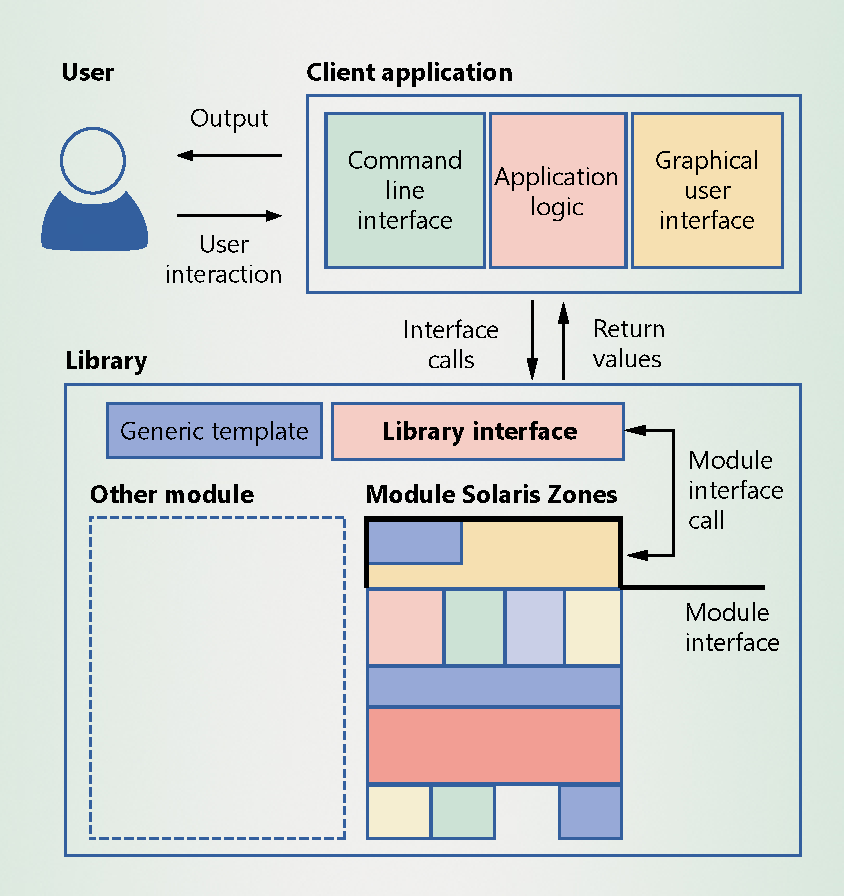
\includegraphics[scale=0.65]{assets/pdfs/architecture.pdf}
    \caption{Architektura funkčních bloku aplikace}
    \label{image:architecture}
\end{figure}
\subsection{Knihovna}
\label{chapter:design:architecture:library}
Knihovna je kontejner, který se bude starat o~zprostředkování komunikace mezi klientem a modulem knihovny. Součástí
knihovny budou jednotlivé moduly, které budou zajišťovat konkrétní funkcionalitu. V~tomto případě se bude jednat o~modul, který
bude implementovat základní funkce pro administraci Solaris Zones. Knihovna pak bude tyto administrační funkce poskytovat klientům.
Celá knihovna bude navržená tak, aby se dala jednoduše rozšířit o~další modul. Tento modul bude muset implementovat určité
rozhraní, pomocí kterého s~ním bude knihovna komunikovat. Díky této architektuře bude v~budoucnu jednoduché implementovat
další modul, který bude zprostředkovávat administraci jiného virtualizačního nástroje. Dalším kandidátem může být například
modul využívající rozhraní aplikace VirtualBox, která také nabízí rozhraní na příkazové řádce.

Mimo funkcí implementovaných v~modulech bude knihovna poskytovat i~některé vlastní funkce. Většina virtualizačních technik
má společnou jednu věc. Tím je specifikace virtuálního stroje, který chce uživatel ve virtualizovaném prostředí spouštět. Tato specifikace
by měla obsahovat základní vlastnost a prostředky, které bude moci daný virtuální stroj využívat. Proto bude knihovna implementovat
generickou šablonu, která bude sloužit pro specifikaci virtuálních strojů. V~podstatě se bude jednat o~hlavičku, která bude určovat
název a typ specifikace. Podle typu této specifikace pak bude knihovna přesměrovávat požadavky na konkrétní modul.

Architektura knihovny bude typu \textit{standalone} a nebude tedy poskytovat žádné rozhraní, které by bylo dostupné z~počítačové
sítě. Veškerou funkcionalitu knihovny bude možné využívat pouze ve stejném systému. Tento krok minimalizuje rizika spojená
s~napadením aplikace prostřednictvím počítačové sítě.
\subsection{Modul Solaris Zones}
\label{chapter:design:architecture:szones}
Jednou z~hlavních částí aplikace bude modul Solaris Zones, který bude součástí výše zmíněné knihovny. Tento modul se bude skládat
z~několika hierarchicky uspořádaných vrstev, které se budou navzájem využívat. Nejníže v~hierarchii se bude nacházet vrstva,
která bude poskytovat spouštění základních nástrojů sloužících pro správu Solaris Zones. Pro poskytnutí základní funkcionality
musí tato vrstva poskytovat následující nástroje:
\begin{itemize}
 \item \verb|zonecfg(1)|,
 \item \verb|zoneadm(1)|,
 \item \verb|zfs(1)|,
 \item \verb|archvieadm(1)|.
\end{itemize}
Tato vrstva bude tedy umožňovat vyšším vrstvám spouštět tyto nástroje s~různým nastavením a různými příkazy.

Vyšší vrstvy budou implementovat základní administrátorské rutiny, které budou složené z~funkcí nižších vrstev. Tento modul
bude zajišťovat smazání všech dočasných souborů, které byly v~průběhu rutiny vytvořeny. K~tomu bude také
zajišťovat konzistenci ve smyslu navrácení všech změn, které byly v~průběhu rutiny provedeny. Toto chování bude nastávat
pouze v~případě, kdy v~průběhu rutiny dojde k~chybě.

Jelikož bude tento modul součástí výše zmíněné knihovny, bude od něj očekávána implementace daného rozhraní. Mimo jiné 
bude muset modul implementovat funkce pro validaci a zpracování šablon, které budou sloužit pro~specifikaci vlastností
neglobálních zón.
\subsection{Klientská aplikace}
\label{chapter:design:architecture:client}
Poslední neméně důležitou částí nástroje pro správu virtualizačního kontejneru Solaris Zones bude klientská aplikace. Tento
funkční blok bude mít za úkol zprostředkovat uživateli funkce modulu Solaris Zones. Samostatná knihovna bude pouze prostředkem,
jakým způsobem přímo spravovat konkrétní zónu. Z~tohoto důvodu bude na klientské aplikaci, aby zařídila možnost správy většího
množství neglobálních zón.

Takto vylepšené možnosti správy Solaris Zones bude klientská aplikace nabízet uživateli pomocí uživatelského rozhraní. Toto
uživatelské rozhraní by mělo být jednoduché a přehledné, ale přitom nabízet nejdůležitější funkce pro správu zón. Klientská
aplikace by si měla udržovat seznam hostů, které chce daný uživatel spravovat. Na základě tohoto seznamu by měla například
zobrazovat všechny neglobální zóny, které se na těchto hostech nachází.

Jelikož aplikaci bude moc využívat více uživatelů, bude každému z~nich poskytovat nezávislý pohled. K~tomuto účelu bude aplikace
využívat uživatelův domovský adresář, kde si bude potřebné informace ukládat. Bude se jednat například o~zóny, se kterými
uživatel nějak manipuloval nebo je vytvářel. Na~základě těchto dat pak klientská aplikace může zobrazovat uživateli změny,
které nastaly v~době jeho nepřítomnosti.
\section{Uživatelské rozhraní}
\label{chapter:design:ui}
Požadavky v~kapitole \ref{chapter:design:demands} stanovují, že hlavním ovládacím prvkem implementované aplikace bude
uživatelské rozhraní. Uživatelské rozhraní je prvek, který uživateli umožňuje konkrétním způsobem interagovat s~danou aplikací.
Tento prvek je možné implementovat pomocí mnoha technologií. Ne všechny typy uživatelského rozhraní jsou však vhodné pro 
konkrétní typy aplikací.

Hlavní podstatou navrhovaného nástroje je podpora automatizace správy. Nástroj má uživateli umožnit zvládnout
hodně práce s~malým množství příkazů. Příkladem může být vytvoření desítek neglobálních zón pomocí jedné akce v~uživatelském 
rozhraní. Dalším požadavkem na uživatelské rozhraní může být i možnost uživatelské rozhraní skriptovat a využívat ho například
v~automatických zálohovacích rutinách. Uživatelské rozhraní tedy musí především umět pracovat v~dávkovém režimu. Musí však
umožňovat i interaktivní instalaci neglobálních zón.

V~dnešní době je pravděpodobně nejpopulárnější webové uživatelské rozhraní. Tento způsob definuje uživatelské rozhraní pomocí
HTML stránek a~pomocí webového serveru nebo Javascriptu, umožňuje reagovat na akce uživatele. Standardně je tento typ uživatelského
rozhraní zprostředkováván pomocí webového serveru bežícího na portech 80 v~případě HTTP nebo 443 v~případě HTTPS. Aplikace
využívající webové rozhraní jsou většinou typu klient-server, kde aplikace běží na serveru. Výhodou je, že klient se
k~serveru připojuje vzdáleně pomocí webového prohlížeče a danou aplikaci nemusí mít nainstalovanou. Nevýhodou je nutnost
uživatelské interakce a špatná možnost skriptování. Z~tohoto důvodu je tento typ uživatelského rozhraní nevhodný pro navrhovaný
nástroj.

Klientská aplikace bude jako uživatelské rozhraní využívat kombinaci CLI a grafického rozhraní. Situace a důvody pro použití
konkrétního typu uživatelského rozhraní jsou vysvětleny níže.
\subsection{CLI}
\label{chapter:design:ui:cli}
Pro umožnění jednoduchého skriptování aplikace bude většina její funkcionality prezentována pomocí rozhraní na příkazové
řádce. Celé rozhraní by mělo mít jednotný tvar a syntaxe jednotlivých příkazů by se neměla moc lišit. Uživatel si jednoduše
bude moci specifikovat cílové zóny a akci, kterou na nich chce provést. Program potom bez dalšího zásahu uživatele provede
danou akci a informuje ho o~jejím výsledku pomocí informačního výpisu.

Po zadání příkazu na příkazové řádce bude běh programu ve většině případů neinteraktivní a nebude tedy vyžadovat žádný 
zásah uživatele. Jedinou výjimku bude tvořit interaktivní instalace zóny, kdy bude použito grafického rozhraní. Po ukončení
běhu aplikace může uživatel opět zadávat další příkazy pomocí příkazové řádky.
\subsection{Grafické rozhraní}
\label{chapter:design:ui:gui}
Grafické rozhraní bude v~aplikaci použito ve dvou případech. Prvním případem je již zmiňovaná interaktivní instalace zón. Při
tomto typu instalace bude uživateli zobrazeno dialogové okno, které slouží jako formulář pro vyplnění atributů zóny popsaných
v~kapitole \ref{chapter:zones:configuration}. Po vyplnění formuláře bude aplikace pokračovat standardním neinteraktivním způsobem.

Výsledný nástroj bude využívat grafické rozhraní ještě v~okamžiku, kdy bude uživatel chtít vytvářet nebo upravovat šablony pro
specifikaci virtuálního stroje. Pro tento účel bude aplikace poskytovat editor, který uživateli pomůže s~vytvořením šablony.
Tento editor se bude opět spouštět pomocí příkazové řádky.

Při výběru grafického rozhraní bude nutné brát ohled na fakt, že aplikace je určená pro platformu Solaris. Jelikož Solaris
není standardní platformou, nemusí být všechny grafické knihovny na této platformě podporovány.
\section{Šablony}
\label{chapter:design:templates}
Podle požadavků specifikovaných v~kapitole \ref{chapter:design:demands}, má aplikace umožňovat vytváření šablon. Šablona slouží
jako předpis pro vytvoření virtuálního stroje. Knihovna popsaná v~kapitole \ref{chapter:design:architecture:library} bude definovat 
generickou šablonu, kterou bude aplikace umět zpracovávat. Knihovna bude muset umět načítat šablony ze souborového systému
a provádět základní validaci. Hlavním obsahem šablony bude její jméno a typ. Podle typu se pak knihovna rozhodne
jakému modulu šablonu předá na zpracování.
\subsection{Šablona Solaris Zones}
\label{chapter:design:templates:zones}
Ve výsledném nástroji bude obsažený pouze modul pro administraci virtualizační techniky Solaris Zones. Tento modul bude
definovat typ šablony, který bude specifikovat neglobální zónu. Opět bude poskytovat funkce pro její validaci, ale oproti
knihovně tuto šablonu bude umět využívat pro tvorbu virtuálních kontejnerů Solaris Zones.

Jak již bylo zmíněno, pro úspěšnou instalaci zóny je třeba provést konfiguraci, instalaci 
softwarových balíků a volitelně i konfiguraci systémových služeb. Aby mohla být zóna ze šablony vytvořena, musí šablona obsahovat
právě tyto části.
\subsubsection{Konfigurace zóny}
\label{chapter:design:templates:zones:configuration}
První část šablony bude obsahovat informace o~konfiguraci zóny. Bude zde tedy specifikováno o~jaký typ zóny se jedná,
jaký typ IP adresy má mít, jaké zdroje mají být zóně delegovány a podobně. Obecně lze říct, že v~této části budou specifikovány
globální atributy zóny popsané v~kapitole \ref{chapter:zones:configuration:global_attributes} a zdroje zóny popsané v~kapitole
\ref{chapter:zones:configuration:resources}. Šablona nebude umožňovat specifikovat všechny atributy a zdroje popsané
v~manuálových stránkách \cite{oracle:manpages:zonecfg}, ale jejich podmnožinu, která je využitelná ve většině případů použití virtualizační
techniky Solaris Zones.
\subsubsection{Softwarové balíky}
\label{chapter:design:templates:zones:manifest}
Další podstatnou částí šablony bude sekce se softwarovými balíky. Balíky, které zde uživatel definuje, budou při instalaci
zóny z~této šablony nainstalovány do kořenového souborového systému zóny. Ihned po prvním startu zóny je uživatel bude moci
využívat. Tato část šablony umožňuje uživateli jasně definovat softwarové vybavení a umožňuje tak vytváření konzistentního
prostředí.

Přehled softwarových balíků dostupných pro konkrétní verzi operačního systému Solaris může uživatel získat pomocí nástroje
pro správu softwarových balíků \verb|pkg(1)| nebo z~oficiálního repozitáře \cite{oracle:solaris:desing:pkg_repository}.
\subsubsection{Systémový profil}
\label{chapter:design:templates:zones:profile}
Poslední sekcí šablony pro definici neglobální zóny je konfigurace systémového profilu. V~této části šablony může uživatel
definovat konfiguraci pro základní systémové služby. Touto cestou může uživatel například nastavovat konfiguraci síťových
adaptérů definovaných v~sekci s~konfigurací. Uživatel může také nastavit časovou zónu, jazyk systému nebo uživatelské účty.
Tato sekce nebude opět umožňovat konfiguraci všech systémových služeb, ale jejich část nutnou ke správné a funkční konfiguraci
systému.

Minimální konfigurace obsahuje definici hesla uživatele \textit{root} a definici počátečního systémového uživatele. Pokud uživatel
nespecifikuje konfiguraci systémových služeb v~šabloně, nebude instalovaná zóna vůbec nakonfigurována. Při prvním spuštění
zóny bude uživatel vyzván k~interaktivní konfiguraci systému.
\section{Automatizace}
\label{chapter:design:automation}
Automatizaci administračních procesů bude aplikace zajišťovat na úrovni modulu, který slouží pro správu Solaris Zones. Pokročilejší
administrační rutiny se skládají ze sekvence několika příkazů, které musí být provedeny po sobě. V~případě selhání, některého
z~nich dojde k~selhání celé rutiny. Často je potřeba při provádění těchto činností vytvořit dočasné soubory nebo dočasně 
vypnout konkrétní zónu. Tyto situace nastávají hlavně v~zálohovacích a migračních rutinách. Modul Solaris Zones bude implementovat
tyto pokročilejší rutiny a poskytovat je skrze knihovnu klientským aplikacím. Dále bude zajišťovat, že všechny dočasné soubory
budou na konci rutiny odstraněny a dočasné akce vráceny v~případě neúspěchu. Toto chování se dá přirovnat k~chování transakcí.

Dále bude příkazová řádka aplikace umožňovat zadávání většího počtu neglobálních zón, pro které se má daný příkaz vykonat. Aplikace
potom paralelně (pokud je to možné) vykoná daný příkaz pro všechny specifikované zóny.
\section{Vzdálená správa}
\label{chapter:design:remote}
Jelikož nástroje pro správu virtualizační techniky Solaris Zones neumožňují správu neglobálních zón na vzdálených serverech,
bude modul zmíněný v~kapitole \ref{chapter:design:architecture:szones} implementovat i funkce pro vzdálenou správu. Ideálním
nástrojem pro ovládání vzdálených serverů je program \verb|ssh(1)|. Tento nástroj umožňuje používat příkazovou řádku na 
vzdáleném serveru a s~použitím veřejného a privátního klíče umožňuje i neinteraktivní přihlášení. Tyto dvě vlastnosti jsou
pro požadovanou funkcionalitu nástroje pro automatickou správu Solaris Zones klíčové.

Prostředí, do kterého je navrhovaná aplikace směřována, se skládá z~několika virtualizačních serverů, které používají operační
systém Solaris. V~rámci těchto serverů je provozována virtualizační technologie Solaris Zones a běží na nich mnoho neglobálních
zón. Klientská aplikace zmíněná v~kapitole \ref{chapter:design:architecture:client} musí implementovat způsob identifikace
těchto zón v~rámci většího počtu serverů. Pomocí tohoto identifikátoru bude uživatel schopný danou zónu specifikovat na příkazové
řádce a provádět s~ní konkrétní akce.

Aplikace bude umožňovat registraci jednotlivých hostů v~rámci dané infrastruktury. Ke každému hostu si aplikace
bude držet přístupové údaje, které má použít při připojování. Tyto údaje budou zahrnovat především uživatelské jméno a 
privátní klíč, který má být použit pro šifrování spojení. Hromadné akce nabízené uživatelským rozhraním se pak budou vztahovat
právě k~registrovaným hostů.
\section{Bezpečnost}
\label{chapter:design:security}
Důležitou součástí návrhu aplikace je její bezpečnost. V~případě nástroje pro~automatickou správu Solaris Zones je nutné věnovat
zabezpečení velkou pozornost. Nástroje specifikované v~kapitole \ref{chapter:design:architecture:szones} totiž při nesprávném
použití mohou způsobit pád systému. V~případě příkazu \verb|zfs(1)| je možné kompletně zničit souborový systém všech neglobálních zón
a způsobit tak chybu systému. Naopak pomocí příkazů \verb|zoneadm(1)| je možné vytvořit takové množství neglobálních zón, že
dojde k~vyčerpání fyzických prostředků globální zóny a následné nefunkčnosti celého systému. Autoři těchto nástrojů na tento
problém mysleli, a proto jsou všechny tyto příkazy přístupné pouze privilegovaným uživatelům. Pro aplikaci to znamená, že ji 
bude moci spouštět pouze uživatel s~konkrétními právy. Operační systém Solaris poskytuje službu RBAC,
která administrátorovi umožňuje jemněji rozdělit práva mezi uživatele \cite{oracle:solaris:desing:rbac}. Pomocí této služby
je možné vytvořit uživatele, který bude
přímo určený pro~správu zón a bude moci používat všechny nástroje stanovené v~\ref{chapter:design:architecture:szones}. Pro~spouštění
aplikace může být použit jeden z~následujících dvou uživatelů:
\begin{itemize}
 \item Uživatel \textbf{root},
 \item Privilegovaný uživatel (\textbf{RBAC}).
\end{itemize}
V~následujících kapitolách jsou popsány důvody, proč není vhodné pro spouštění aplikace používat uživatele \textit{root} a 
jaké výhody přináší RBAC.
\subsection{Uživatel root}
\label{chapter:design:security:root}
Uživatel \textit{root} je plně privilegovaný uživatel v~rámci operačního sytému Solaris a má potřebná práva pro spouštění všech
potřebných nástrojů. Existuje však několik důvodů, proč není vhodné uživatele \textit{root} používat pro spouštění navrhovaného
nástroje pro automatickou správu Solaris Zones. Jedním z~důvodů je ctění principu nejnižších privilegií 
\cite{cvut:presentations:least_user_privilege}. Tento princip říká, že aplikace má být spuštěna pouze s~nejmenší možnou množinou
práv, se kterými je ještě schopná plnit svůj účel. Pokud by byla aplikace nějakým způsobem zkompromitována, útočník může využít
pouze těchto práv. Pokud by nebyl dodržen princip nejnižších oprávnění a aplikace by byla spouštěna pod uživatelem \textit{root},
útočník by mohl využívat privilegovaného přístupu v~celém systému.

Dalším důvodem proč nepoužívat uživatele \textit{root} je standardní systémové nastavení operačního systému Solaris. Standardně
je totiž uživatel \textit{root} v~systému zaregistrovaný jako role. Role je funkcionalita RBAC \cite{oracle:solaris:desing:rbac},
která se chová téměř jako uživatel. Je možné ji přiřazovat práva na provádění privilegovaných operací nebo se na ní přepínat pomocí
nástroje \verb|su(1)|. Uživatel může mít v~systému přiřazeny role, které může používat. Samotná role však nemá v~systému žádnou
funkci a nedá se na ni dokonce ani přihlásit. Z~tohoto důvodu by nebylo možné přihlašovat se na vzdálených systémech jako uživatel
\textit{root} a~aplikace by nesplňovala požadavek vzdálené správy.

Poslední důvod souvisí s~předchozím důvodem a opět se týká standardního nastavení. Tentokrát se však týká standardního nastavení nástroje
\verb|ssh(1)|, které nepovoluje vzdálené přihlašování uživatele \textit{root}.

V~důsledku používání uživatele \textit{root} by došlo k~porušení principu nejnižších privilegií 
\cite{cvut:presentations:least_user_privilege} a navíc by muselo dojít k~vypnutí některých standardních bezpečnostních opatření.
Z~výše uvedených důvodů není vhodné tohoto uživatele používat pro spouštění navrhovaného nástroje pro automatickou správu Solaris Zones.
\subsection{RBAC}
\label{chapter:design:security:rbac}
Správnou volbou je vytvořit uživatele, kterému pomocí RBAC přiřadíme potřebná oprávnění pro používání potřebných nástrojů.
Aplikace bude spouštěna v~souladu s~principem nejnižších oprávnění a nebude nutné vypínat bezpečnostní
opatření nástroje \verb|ssh(1)| ani jiné systémové nastavení.